\newpage
\subsection{Melihat Kotak Pesan}
Halaman ini hanya dapat diakses oleh pengguna yang sudah terdaftar dan masuk/\textit{login} ke dalam sistem. Pada halaman ini terdapat elemen-elemen halaman \textit{chatting} pada umumnya, yaitu elemen \textit{input} pesan, tombol Kirim, dan riwayat beberapa pesan sebelumnya. Spesifikasi kasus penggunaan dapat dilihat pada Tabel \ref{uc04.05}.\\
\indent Terdapat logika \textit{view} dan alur proses khusus dikarenakan sifat pengiriman dan penerimaan pesan yang \textit{realtime}, sehingga dibangun diatas Node.js dan menggunakan Socket.io. Masing-masing logika tersebut dapat dijabarkan sebagai berikut:
\begin{enumerate}
	\item Logika \textit{back-end} ditulis menggunakan PHP yang dicantumkan dalam Kode Sumber \ref{cdbe.04-05}; dan
	\item Logika \textit{view} ditulis menggunakan Vue.js yang dicantumkan dalam Kode Sumber \ref{cdve.04-05};
\end{enumerate}

\begin{figure}[H]
	\centering
	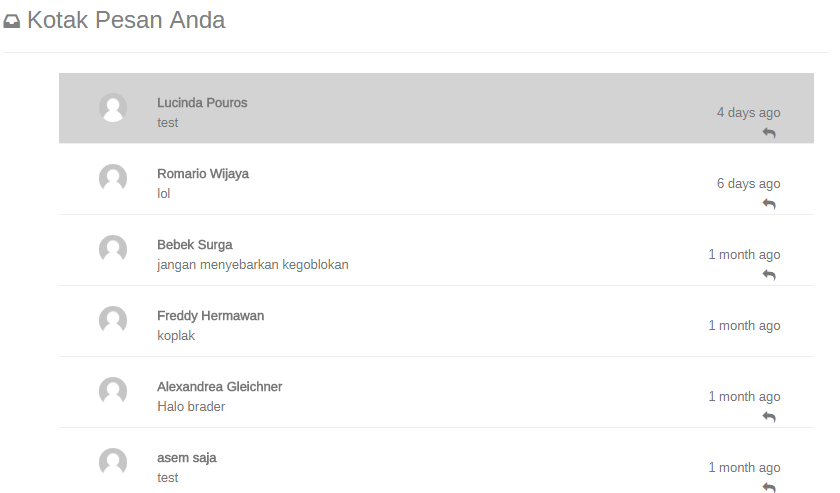
\includegraphics[width=\textwidth]{images/bab4/ui/04-05.png}
	\caption{Halaman Antarmuka Melihat Kotak Pesan}
	\label{ui.04-05}
\end{figure}
\newpage
\begin{lstlisting}[label=cdbe.04-05,style=php,caption=Implementasi \textit{Back-end} Melihat Kotak Pesan]
/*	file : app/Http/Controllers/InboxController */
/* fungsi ini dipanggil saat mengakses url inbox/data */
public function retrieveInbox($id = false)
{
    $r =  $this->chatRep->conversations(
      $id ?
       User::findOrFail($id) :
       Auth::user()
    );

    return response()
        ->json($r);
}

/* file : ChatRepository */
/* fungsi ini dipanggil saat mengakses url inbox/lastDetail */
public function conversations(User $user)
{
    $this->chatroom->setIdComp($user->id);
     return $this->chatroom
			->where('id_user_1',strval($user->id))
             ->orWhere('id_user_2',strval($user->id))
             ->with('friend')
             ->orderBy('updatedAt','desc')
             ->get();
}

public static function getLastChatDetail(User $user, $room)
{
  $res = DB::connection('mongodb')
          ->collection('userchat')
          ->where('room', $room)
          ->orderBy('sent','desc')
          ->first(['msg','sender','sent']);
  $partner = explode("-", $room);
  $partner = $partner[0] != $user->id ? $partner[0] : $partner[1];
  return ( [
      'msg' => $res['msg'],
      'sent' => $res['sent'] ?
        	( new Carbon($res['sent']->toDateTime()
	            ->format('r')))
	            ->diffForHumans() 
        	   : "Unknown",
      'partner' => $partner,
      'isSender' => $res['sender'] == $user->id
  ]);

}

\end{lstlisting}

\begin{lstlisting}[label=cdve.04-05,style=htmlcssjs,caption=Implementasi Logika \textit{View} Lihat Kotak Pesan (menggunakan Node.js)]
<template>
    <ul class="friend-list table-hover table-responsive" v-if="conversations.length>0 && loaded">
      <li  v-for="(conv, index) in conversations">
        <a v-bind:href="getUrl(det[index].partner)" class="clearfix">
          <div class="col-sm-12">
           <div class="col-sm-1">
             <img src="url_image_default" alt="" class="img-circle">
           </div>
           <div class="col-sm-11">
             <div class="friend-name">
               <strong>{{ conv.friend.name }}</strong>
             </div>
             <div class="last-message text-muted">
                 <!--i want to show last chat here-->
               {{ det[index].msg }}
             </div>
             <small class="time text-muted">
                 <!-- i want to show the msg timestamp here-->
               {{ det[index].sent }}
             </small>
             <small class="chat-alert text-muted">
               <i v-if="det[index].isSender" class="fa fa-reply"></i>
             </small>
           </div>
          </div>
        </a>
      </li>
    </ul>
    <ul class="friend-list" v-else>
      <li>
         <div class="friend-name">
             No messages!
         </div>
      </li>
    </ul>w
</template>

<script>
    export default
    {
     props: ['id'],
     data: function () {
       return {
         conversations: [],
         det : [],
         loaded : false
       }
     },
     created() {
      axios.get('/inbox/data')
      .then(response => {
        //fetching conversations id and its detail

        this.conversations = response.data;

        var promises = [];

        response.data.forEach(conv => {
          promises.push(
           axios.post('/inbox/lastDetail',{
             room : conv.room
           })
          )
        });

        axios.all(promises).then( results => {
          this.det = results.map(result => result.data);
          this.loaded = true;
        })
      });
     },
     methods: {
      getUrl(id){
       return ("https://lelangapa.com/chat/" + id);
      }
     }
    }
</script>
\end{lstlisting}